\documentclass[11pt]{article}

\usepackage[a4paper, margin=1.05in]{geometry}
\usepackage{amsmath, amssymb, amsthm, mathtools}
\usepackage{graphicx}
\usepackage{booktabs}
\usepackage{microtype}
\usepackage{xcolor}
\usepackage{enumitem}
\usepackage[normalem]{ulem}
\usepackage[hypertexnames=false]{hyperref}
\hypersetup{colorlinks=true, linkcolor=black!55!blue, urlcolor=black!45!blue}
\sloppy \emergencystretch=2.5em

\theoremstyle{plain}
\newtheorem{lemma}{Lemma}
\newtheorem{proposition}{Proposition}
\newtheorem{theorem}{Theorem}
\theoremstyle{remark}
\newtheorem{remark}{Remark}

\newcommand{\R}{\mathbb{R}}
\newcommand{\N}{\mathcal{N}}
\newcommand{\E}{\mathbb{E}}
\newcommand{\Z}{\mathcal{Z}}
\newcommand{\dd}{\mathrm{d}}
\newcommand{\T}{^{\!\top}}
\newcommand{\one}{\mathbf{1}}
\newcommand{\score}{s}
\DeclareMathOperator{\tr}{tr}
\DeclareMathOperator*{\argmax}{arg\,max}

\title{The three board problems\\[2pt]
\large Rotating rings, two-frame joints, and terminal rewards}
\author{Working note}
\date{25 July 2026}

\begin{document}
\maketitle

\begin{abstract}
\noindent
Three problems were circled on the board: a rotating point near a ring whose
whole trajectory is one data point, the two-frame joint law and its Gaussian
closed form, and a reward on the last frame propagated backwards. This note
develops all three in the simplest setting that keeps their content, shows every
computation, and states plainly which claims are proved, which are measured, and
which turned out to be false. The central technical result is that the rotating
ring model --- previously recorded as having no closed-form joint score --- is
exactly solvable: the rotation is a gauge, the ring is a location mixture, and
the joint score is a linear part plus a rank-one correction obtained from one
one-dimensional Bessel integral. Two scaling claims made in a first pass are
rejected here by measurement.
\end{abstract}

\tableofcontents

%======================================================================
\section{The setting, and why the joint}\label{sec:setting}

\subsection{Two clocks}

Everything in this note has two time variables and keeping them apart is the
whole discipline of the problem.

\begin{itemize}[leftmargin=1.4em, itemsep=2pt]
\item The \emph{internal} time $u = 0, 1, \dots, T-1$ indexes position along a
      trajectory. On the board it appears as $u \in [0, 2\pi/\omega]$ with the
      working value $T = 40$.
\item The \emph{diffusion} time $t$ indexes the noise level of the generative
      channel.
\end{itemize}

A data point is not a frame. It is a \emph{whole trajectory},
\begin{equation}
  a = \bigl(x(0), y(0), x(1), y(1), \dots, x(T{-}1), y(T{-}1)\bigr) \in \R^{2T},
  \qquad D = 2T,
  \label{eq:a}
\end{equation}
exactly as the board writes it, $a^\mu = \{x^\mu(u), y^\mu(u)\}$. The forward
channel is the variance-preserving Ornstein--Uhlenbeck channel,
\begin{equation}
  x = m\, a + \sqrt{\Delta}\, \xi, \qquad
  m = e^{-t}, \quad \Delta = 1 - e^{-2t}, \quad \xi \sim \N(0, I_D),
  \label{eq:channel}
\end{equation}
and it acts on \emph{all} of $a$ at once. That single fact is why the object of
study is the \emph{joint} score
\begin{equation}
  \score(x,t) = \nabla_x \log P_t(x), \qquad
  P_t(x) = \int \dd a\, P_0(a)\, \N(x; m a, \Delta I_D),
  \label{eq:score}
\end{equation}
the board's $\score(x,t) \to \nabla \log (P_0 \circledast G)$, and not a
collection of per-frame scores. Figure~\ref{fig:twoclocks} shows the two clocks
acting on one trajectory: the internal time runs along the curve, the diffusion
time destroys it.

\begin{figure}[t]\centering
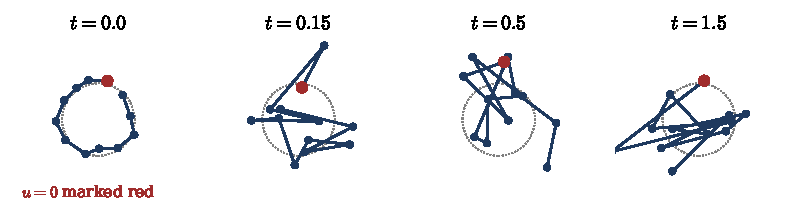
\includegraphics[width=\linewidth]{fig01_two_clocks.pdf}
\caption{The two clocks. One trajectory of the rotating ring model
($T = 12$, $\sigma = 0.10$, $\psi = 2\pi/12$), shown at four diffusion times
$t$. The internal time $u$ runs along the polyline, from the red dot. The
diffusion time $t$ shrinks the whole trajectory towards the origin and blurs it;
at $t = 1.5$ nothing of the dynamics survives. The dotted circle is the unit
ring.}
\label{fig:twoclocks}
\end{figure}

\subsection{The score--posterior identity}

We use one standard identity throughout. Differentiating \eqref{eq:score},
\begin{equation}
  \nabla_x P_t(x) = \int \dd a\, P_0(a)\, \N(x; ma, \Delta I)\,
  \frac{m a - x}{\Delta},
\end{equation}
so dividing by $P_t(x)$,
\begin{equation}
  \boxed{\ \score(x,t) = \frac{m\,\E[a \mid x] - x}{\Delta}\ }
  \label{eq:tweedie}
\end{equation}
where the expectation is over the posterior of the clean trajectory given the
noisy one. The score is a denoiser. Every closed form below is, at bottom, a
posterior mean that happens to be computable.

%======================================================================
\section{Problem 1: the rotating ring}\label{sec:p1}

\subsection{The model}

The board's left panel. Three latent variables, independent:
\begin{equation}
  r_0 \sim p_\lambda(\rho) \propto \rho\, e^{-(\rho-1)^2/2\lambda},
  \qquad \theta_0 \sim \mathrm{Unif}[0, 2\pi), \qquad \psi \sim p(\psi),
  \label{eq:latents}
\end{equation}
and then
\begin{equation}
  z_0 = r_0(\cos\theta_0, \sin\theta_0), \qquad
  z_{u+1} = R_\psi z_u + \sigma \eta_{u+1}, \qquad
  \eta_u \sim \N(0, I_2)\ \text{i.i.d.}
  \label{eq:chain}
\end{equation}
Here $R_\psi$ is planar rotation by $\psi = \omega \Delta u$. The factor $\rho$
in $p_\lambda$ is the two-dimensional area element: the density of the point
$z_0 \in \R^2$ is $\propto e^{-(\|z\|-1)^2/2\lambda}$, so its radial marginal
carries an extra $\rho$. Figure~\ref{fig:ring} checks the sampler against this.

\eqref{eq:chain} is the discrete form of the pair written on the board,
$\dd r = (1-r)\dd u + \Gamma \dd B_u$ from the potential
$V(r) = \tfrac12 (r-1)^2$, together with $\dot\theta = \omega$.

At $T = 2$ the data vector is the board's own
$(x_0, y_0, x_1, y_1) = a^\mu \in \R^4$. With three latents in ambient dimension
four, this is the board's ``$\rho$ dim 3''. That is the setting we use.

\begin{figure}[t]\centering
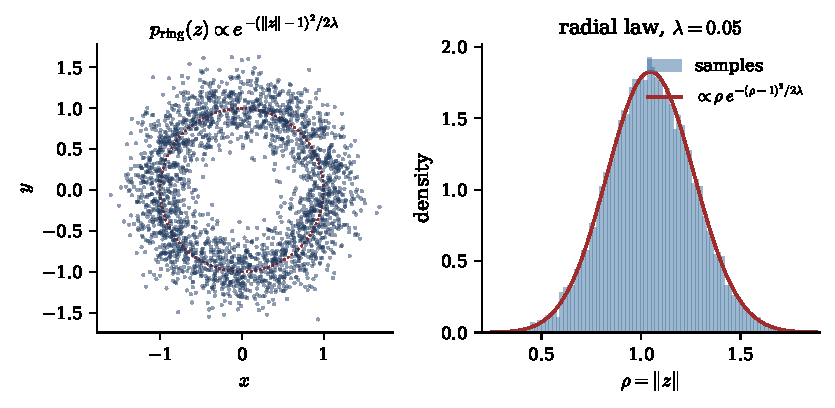
\includegraphics[width=\linewidth]{fig02_ring.pdf}
\caption{The ring prior, $\lambda = 0.05$. Left: $2500$ draws of $z_0$ with the
unit circle dotted. Right: the histogram of $\rho = \|z_0\|$ from $20\,000$
draws against the radial density $\propto \rho\, e^{-(\rho-1)^2/2\lambda}$. The
mode sits slightly outside $\rho = 1$ because of the area element.}
\label{fig:ring}
\end{figure}

\subsection{The symmetry}

$P_0$ is invariant under rotating \emph{every} frame by the same angle,
$\mathcal{R}_\phi = \mathrm{blockdiag}(R_\phi, \dots, R_\phi)$. Indeed
$\mathcal{R}_\phi a$ is the trajectory built from
$(r_0, \theta_0 + \phi, \psi)$, and $\theta_0$ is uniform. Since the channel
\eqref{eq:channel} is isotropic, $P_t$ inherits the invariance for every $t$,
and the score is equivariant,
\begin{equation}
  \score(\mathcal{R}_\phi x, t) = \mathcal{R}_\phi\, \score(x, t).
  \label{eq:equivariance}
\end{equation}
This is the board's boxed $R_\psi(x)$ statement. It has a strong consequence,
Theorem~\ref{thm:blind} below.

\subsection{Step 1: the rotation is a gauge}

\begin{lemma}[Gauge reduction]\label{lem:gauge}
Let $U_\psi = \mathrm{blockdiag}(R_{-u\psi})_{u=0}^{T-1} \in O(2T)$. Then
$U_\psi a$ has the law of the same model with $\psi = 0$, i.e.\ a planar random
walk started on the ring. Consequently, writing $P_t^0$ and $\score^0$ for the
$\psi = 0$ quantities,
\begin{equation}
  P_t(x \mid \psi) = P_t^0(U_\psi x), \qquad
  \score(x, t \mid \psi) = U_\psi\T \score^0(U_\psi x, t).
  \label{eq:gauge}
\end{equation}
\end{lemma}

\begin{proof}
Put $\tilde z_u = R_{-u\psi} z_u$. Then from \eqref{eq:chain}
\begin{equation}
  \tilde z_{u+1}
  = R_{-(u+1)\psi}\bigl(R_\psi z_u + \sigma \eta_{u+1}\bigr)
  = R_{-u\psi} z_u + \sigma R_{-(u+1)\psi}\eta_{u+1}
  = \tilde z_u + \sigma \tilde\eta_{u+1},
\end{equation}
with $\tilde\eta_{u+1} = R_{-(u+1)\psi}\eta_{u+1}$. A rotation of an isotropic
Gaussian is the same isotropic Gaussian, and the $\tilde\eta_u$ remain
independent, so $\tilde z$ is a random walk with step $\sigma$; and
$\tilde z_0 = z_0$ still sits on the ring.

For the second claim, $U_\psi$ is orthogonal, so applying it to
\eqref{eq:channel} gives
$U_\psi x = m\,U_\psi a + \sqrt{\Delta}\,U_\psi \xi$ with
$U_\psi \xi \sim \N(0, I)$. Hence $U_\psi x$ has exactly the law of the noisy
$\psi = 0$ model, and since $|\det U_\psi| = 1$ the densities satisfy
$P_t(x \mid \psi) = P_t^0(U_\psi x)$. Differentiating by the chain rule gives
the score identity.
\end{proof}

\begin{remark}
At known $\psi$ the rotation contributes \emph{zero} statistical difficulty: it
is a known orthogonal change of frame. Everything hard about the model is a
random walk anchored on a ring. Figure~\ref{fig:gauge} shows the two frames.
\end{remark}

\begin{figure}[t]\centering
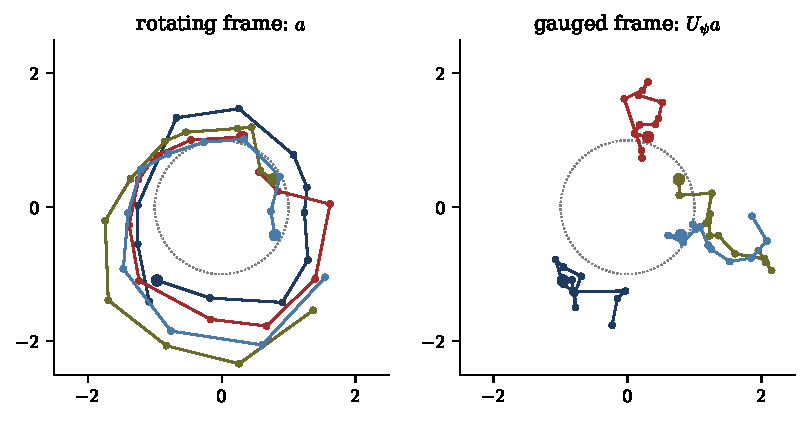
\includegraphics[width=\linewidth]{fig03_gauge.pdf}
\caption{The gauge, on four trajectories ($T = 12$, $\sigma = 0.22$,
$\psi = 30^\circ$; large dots mark $u = 0$). Left: the data, coherently
circulating. Right: the same trajectories after $U_\psi$. The circulation is
gone and what remains is a random walk started on the ring. $U_\psi$ is
orthogonal, so it commutes with the isotropic channel and this reduction is
exact at every diffusion time.}
\label{fig:gauge}
\end{figure}

\subsection{Step 2: the ring is a location mixture}

Work in the gauged frame and write the trajectory as a matrix
$X \in \R^{T\times 2}$, row $u$ being frame $u$. From
$\tilde z_u = z_0 + \sigma\sum_{k\le u}\eta_k$ we get, \emph{conditionally on
$z_0$}, a Gaussian with
\begin{equation}
  \E[\tilde z_u \mid z_0] = z_0, \qquad
  \mathrm{Cov}(\tilde z_u, \tilde z_v \mid z_0) = \sigma^2 \min(u,v)\, I_2 .
\end{equation}
So with $K_{uv} = \min(u,v)$ the conditional law of the trajectory is
$\N(\one z_0\T,\ \sigma^2 K \otimes I_2)$, and after the channel
\begin{equation}
  X \mid z_0 \ \sim\ \N\bigl(m\,\one z_0\T,\ A_t \otimes I_2\bigr),
  \qquad
  \boxed{\ A_t = m^2\sigma^2 K + \Delta I_T\ }
  \label{eq:At}
\end{equation}
The point is that $A_t$ \emph{does not depend on $z_0$}. So $P_0$, and $P_t$, is
a two-parameter \emph{location} mixture of a single Gaussian --- the easiest kind
of mixture there is.

\subsection{Step 3: the exact joint score}

\begin{theorem}[Exact joint score, any $T$]\label{thm:score}
Let $g = A_t^{-1}\one$, $\kappa_t = \one\T g$, $b = X\T g \in \R^2$,
$\beta = \|b\|$ and $\hat b = b/\beta$. Then
\begin{equation}
  \log P_t(X) = c(t) - \tfrac12 \tr\bigl[X\T A_t^{-1} X\bigr]
  + \log \Z_t(\beta),
  \label{eq:logpt}
\end{equation}
\begin{equation}
  \Z_t(\beta) = \int_0^\infty \rho\, e^{-(\rho-1)^2/2\lambda}\,
  e^{-m^2\kappa_t \rho^2/2}\, I_0(m\rho\beta)\, \dd\rho,
  \label{eq:Zt}
\end{equation}
and therefore
\begin{equation}
  \boxed{\ \score(X,t) = -A_t^{-1} X + \Phi_t(\beta)\, g\, \hat b\T,
  \qquad \Phi_t = \partial_\beta \log \Z_t\ }
  \label{eq:mainscore}
\end{equation}
a linear part plus a \emph{rank-one} correction.
\end{theorem}

\begin{proof}
Start from the mixture and expand the quadratic form in the exponent. Using
$\tr[M\T N]$ for the Frobenius pairing,
\begin{align}
  \tr\bigl[(X - m\one z_0\T)\T A_t^{-1}(X - m\one z_0\T)\bigr]
  &= \tr[X\T A_t^{-1} X]
   - 2m\, \tr\bigl[z_0 \one\T A_t^{-1} X\bigr]
   + m^2 \tr\bigl[z_0 \one\T A_t^{-1}\one z_0\T\bigr] \notag\\
  &= \tr[X\T A_t^{-1} X] - 2m\, b \cdot z_0 + m^2 \kappa_t \|z_0\|^2,
  \label{eq:expand}
\end{align}
because $\tr[z_0\one\T A_t^{-1}X] = \one\T A_t^{-1} X z_0 = b\cdot z_0$ and
$\tr[z_0 \one\T A_t^{-1}\one z_0\T] = \kappa_t \|z_0\|^2$. Hence
\begin{equation}
  P_t(X) = c(t)\, e^{-\frac12 \tr[X\T A_t^{-1}X]}
  \int_{\R^2} \dd z_0\; e^{-(\|z_0\|-1)^2/2\lambda}\;
  e^{\,m\, b\cdot z_0 \;-\; \frac12 m^2 \kappa_t \|z_0\|^2}.
  \label{eq:mixint}
\end{equation}
Now the integral is two-dimensional and its integrand depends on the direction
of $z_0$ only through $b\cdot z_0$. Put $z_0 = \rho(\cos\phi, \sin\phi)$ so that
$\dd z_0 = \rho\,\dd\rho\,\dd\phi$ and
$b \cdot z_0 = \rho\beta\cos(\phi - \arg b)$. The angular integral is the
standard integral representation of the modified Bessel function,
\begin{equation}
  \int_0^{2\pi} e^{\,m\rho\beta\cos(\phi - \arg b)}\, \dd\phi
  = 2\pi\, I_0(m\rho\beta),
\end{equation}
which leaves exactly $2\pi\,\Z_t(\beta)$ of \eqref{eq:Zt} and proves
\eqref{eq:logpt}.

For the gradient, the first term of \eqref{eq:logpt} gives $-A_t^{-1}X$. For the
second, $b_j = \sum_u g_u X_{uj}$, so $\partial b_j/\partial X_{ui} =
\delta_{ij} g_u$ and
\begin{equation}
  \frac{\partial \beta}{\partial X_{ui}}
  = \frac{b_j}{\beta}\frac{\partial b_j}{\partial X_{ui}} = g_u \hat b_i .
\end{equation}
Therefore $\nabla_X \log\Z_t(\beta) = \Phi_t(\beta)\, g\,\hat b\T$, an outer
product, hence rank one.
\end{proof}

So for \emph{any} number of frames the exact joint score costs one
one-dimensional integral. Two readings of the correction term:

\begin{proposition}[The correction is the denoised anchor]\label{prop:anchor}
$\Phi_t(\beta)\,\hat b = m\, \E[z_0 \mid X, t]$.
\end{proposition}

\begin{proof}
By \eqref{eq:mixint} the posterior of $z_0$ given $X$ is
$\propto e^{-(\|z_0\|-1)^2/2\lambda} e^{m b\cdot z_0 - \frac12 m^2\kappa_t\|z_0\|^2}$.
Its normalisation is $2\pi\Z_t(\beta)$, which depends on $b$ only through
$\beta = \|b\|$. Differentiating the log-normalisation with respect to $b$ pulls
out exactly $m$ times the posterior mean:
$\nabla_b \log \Z_t(\|b\|) = m\,\E[z_0\mid X]$. But
$\nabla_b = \hat b\, \partial_\beta$, so
$\Phi_t(\beta)\hat b = m\E[z_0 \mid X]$.
\end{proof}

That is why the correction is rank one and why it points along $\hat b$: it is
the single denoised ring anchor, broadcast to every frame with weights $g$.
Figure~\ref{fig:phi} plots $\Phi_t$ and the anchor radius $\Phi_t/m$: at small
$t$ the anchor sits on the ring, $\|\E[z_0\mid x]\| \to 1$; at large $t$ the
posterior collapses to the origin.

\begin{figure}[t]\centering
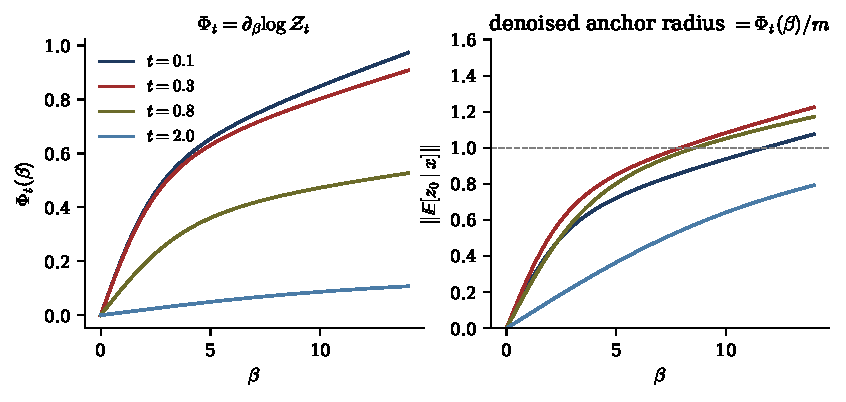
\includegraphics[width=\linewidth]{fig05_phi.pdf}
\caption{The scalar function that carries all the non-Gaussianity ($T = 6$,
$\sigma = 0.30$, $\lambda = 0.05$). Left: $\Phi_t(\beta) = \partial_\beta
\log\Z_t$. Right: the same divided by $m$, which by
Proposition~\ref{prop:anchor} is the length of the posterior mean of the ring
anchor. It saturates at $1$ (dashed) --- once the data pin the anchor, it sits
on the unit ring.}
\label{fig:phi}
\end{figure}

\subsection{The band structure of \texorpdfstring{$A_t^{-1}$}{At inverse}}

$A_t$ is where the temporal structure lives, so its inverse is worth looking at.

\begin{proposition}\label{prop:band}
$K_{uv} = \min(u,v)$ has rank $T-1$ and vanishing $0$th row, so
\begin{enumerate}[label=(\alph*), leftmargin=1.9em, itemsep=1pt]
\item $A_t$ is exactly block diagonal, $[\Delta] \oplus (\text{rest})$: frame
      $0$ decouples in $A_t^{-1}$ at every $t$;
\item on the remaining block the $d$th off-diagonal of $A_t^{-1}$ is of order
      $(\Delta/m^2\sigma^2)^d$, so $A_t^{-1}$ becomes tridiagonal as
      $t \to 0$.
\end{enumerate}
\end{proposition}

Part (a) is not an accident: frame $0$ \emph{is} $z_0$ and carries no walk noise,
so conditionally on $z_0$ it has zero variance and its only spread is the
diffusion $\Delta$. Note this also means $A_0^{-1}$ does not exist; an earlier
draft of this note asserted ``$A_0^{-1} = K^{-1}/\sigma^2$ is tridiagonal'',
which is meaningless. Part (b) is the correct statement, and it is the band-fill
law of the Gaussian chain (claim G8 of the main thesis ledger) in this model,
with small parameter $\Delta/m^2\sigma^2$. Figure~\ref{fig:band} measures it.

\begin{figure}[t]\centering
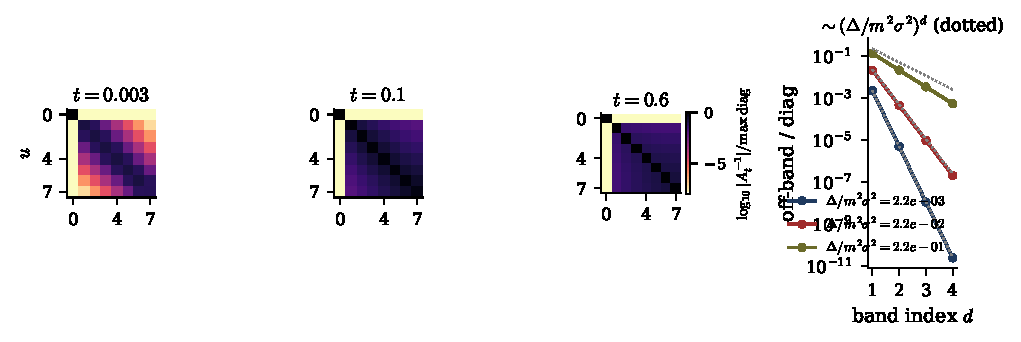
\includegraphics[width=\linewidth]{fig06_bandfill.pdf}
\caption{Band structure of $A_t^{-1}$ ($T = 8$, $\sigma = 0.30$). First three
panels: $\log_{10}$ of $|A_t^{-1}|$ normalised by its largest diagonal entry.
Frame $0$ is decoupled at every $t$ (white cross), exactly. Right: the $d$th
off-band, normalised, against the prediction $(\Delta/m^2\sigma^2)^d$ (dotted).
The law holds over eleven decades.}
\label{fig:band}
\end{figure}

\subsection{Step 4: a random rotation rate}

The board wants $\omega$ drawn per sample. That costs one more one-dimensional
integral and nothing else.

\begin{proposition}[Random $\psi$]\label{prop:mix}
For any $T$,
\begin{equation}
  \score(x,t) = \int \dd\psi\; p(\psi \mid x, t)\;
  U_\psi\T\, \score^0(U_\psi x, t),
  \qquad
  p(\psi \mid x,t) \propto p(\psi)\, P_t^0(U_\psi x).
  \label{eq:mixscore}
\end{equation}
\end{proposition}

\begin{proof}
$P_t(x) = \int p(\psi) P_t(x\mid\psi)\dd\psi$, so
\begin{equation}
  \nabla \log P_t
  = \frac{\int p(\psi)\, \nabla P_t(x\mid\psi)\,\dd\psi}{P_t(x)}
  = \int \frac{p(\psi) P_t(x\mid\psi)}{P_t(x)}\,
    \nabla\log P_t(x\mid\psi)\,\dd\psi,
\end{equation}
which is \eqref{eq:mixscore} after inserting Lemma~\ref{lem:gauge}.
\end{proof}

Combining Theorem~\ref{thm:score} and Proposition~\ref{prop:mix}: the full board
model has \textbf{ground-truth score at any $T$ from two nested
one-dimensional quadratures} --- the $\psi$ integral outside, the Bessel
integral inside. No network, no Monte Carlo, no curse of dimension. This is the
tool everything below uses.

\subsection{At two frames the posterior simplifies}

\begin{proposition}\label{prop:T2}
At $T = 2$ only, $A_t = \mathrm{diag}(\Delta_1, \Delta_2)$ with
$\Delta_1 = \Delta$, $\Delta_2 = m^2\sigma^2 + \Delta$, and
\begin{equation}
  p(\psi\mid x, t) \propto p(\psi)\, \Z_t(\beta(\psi)),
  \qquad
  \beta(\psi)^2 = \frac{|x_0|^2}{\Delta_1^2} + \frac{|x_1|^2}{\Delta_2^2}
  + \frac{2 |x_0| |x_1| \cos(\gamma - \psi)}{\Delta_1\Delta_2},
  \label{eq:betapsi}
\end{equation}
where $\gamma = \arg x_1 - \arg x_0$ is the observed turning angle. The data
enter only through $(|x_0|, |x_1|, \gamma)$, and the posterior is unimodal with
its peak at $\psi = \gamma$.
\end{proposition}

\begin{proof}
For $T = 2$, $K = \mathrm{diag}(0,1)$, so $A_t$ is diagonal as stated. Then
\begin{equation}
  \tr\bigl[(U_\psi X)\T A_t^{-1}(U_\psi X)\bigr]
  = \sum_u \frac{\|R_{-u\psi}x_u\|^2}{(A_t)_{uu}}
  = \sum_u \frac{\|x_u\|^2}{(A_t)_{uu}},
\end{equation}
which is $\psi$-free because rotations preserve norms. So in \eqref{eq:logpt}
only $\log\Z_t(\beta(\psi))$ depends on $\psi$, giving the first claim. For the
second, use complex coordinates: $b = x_0/\Delta_1 + e^{-i\psi}x_1/\Delta_2$, so
\begin{equation}
  |b|^2 = \frac{|x_0|^2}{\Delta_1^2} + \frac{|x_1|^2}{\Delta_2^2}
  + \frac{2}{\Delta_1\Delta_2}\,\mathrm{Re}\bigl(\bar x_0 e^{-i\psi} x_1\bigr),
\end{equation}
and $\mathrm{Re}(\bar x_0 e^{-i\psi}x_1) = |x_0||x_1|\cos(\gamma - \psi)$.
Finally $\Z_t$ is a positive mixture of $I_0(m\rho\beta)$, each increasing in
$\beta$, so $\Z_t$ increases in $\beta$, and $\beta(\psi)$ is maximised at
$\psi = \gamma$.
\end{proof}

\begin{remark}[Scope]\label{rem:scope}
The simplification is genuinely special to $T = 2$. $U_\psi$ conjugates
$A_t \otimes I_2$ into itself if and only if $A_t$ is diagonal in $u$, and
$K_{uv} = \min(u,v)$ is diagonal only for $T = 2$. For $T \ge 3$ the cross terms
$x_u \cdot R_{(u-v)\psi} x_v$ survive and the quadratic form does depend on
$\psi$; measured, the spread is $10$--$13\%$ at $T = 3, 5$. The audit tests both
sides of this boundary. Proposition~\ref{prop:mix} is unaffected --- it is
Bayes, and holds for all $T$.
\end{remark}

Figure~\ref{fig:psipost}, left, is \eqref{eq:betapsi} in action: a bump on the
observed turning angle that widens as the noise rises.

\begin{figure}[t]\centering
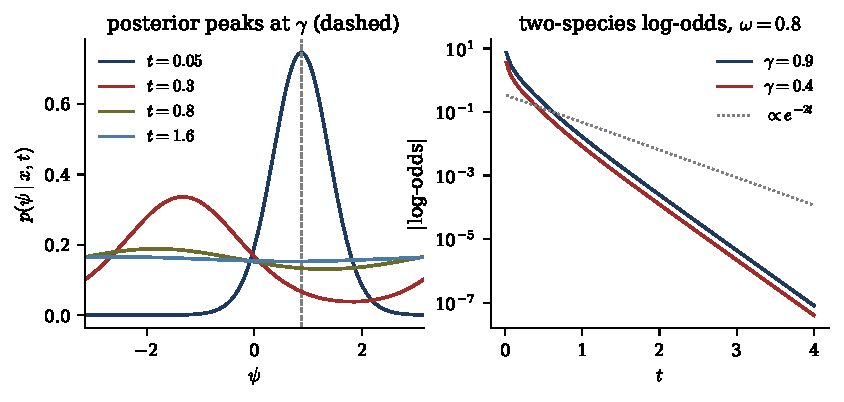
\includegraphics[width=\linewidth]{fig07_psi_posterior.pdf}
\caption{Left: the $\psi$-posterior at $T = 2$ for one data point, at four
diffusion times. It peaks at the observed turning angle $\gamma$ (dashed) and
flattens as $t$ grows: the dynamics are being forgotten. Right: the two-species
log-odds of \eqref{eq:logodds} for two values of the true turning angle,
against the predicted $e^{-2t}$ decay (dotted). A trajectory with
$\gamma = 0.4$ is intrinsically harder to classify than one with
$\gamma = 0.9$, as the $\sin\gamma$ factor requires.}
\label{fig:psipost}
\end{figure}

\subsection{Speciation: committing to a sense of rotation}

Take two species, clockwise and counter-clockwise,
$p(\psi) = \tfrac12(\delta_{+\omega} + \delta_{-\omega})$. By
Proposition~\ref{prop:T2} the order parameter is one scalar,
\begin{equation}
  \mathrm{logit}\, \Pr(\psi = +\omega \mid x, t)
  = \log \Z_t(\beta(+\omega)) - \log\Z_t(\beta(-\omega)).
  \label{eq:logodds}
\end{equation}
Its small-$m$ form follows from $I_0(z) = 1 + z^2/4 + O(z^4)$: writing
$N_0 = \int\rho\, g$, $\langle\rho^2\rangle = \int\rho^3 g / \int \rho\, g$ with
$g(\rho) = e^{-(\rho-1)^2/2\lambda}$,
\begin{equation}
  \Z_t(\beta) = N_0\Bigl[1 + m^2\Bigl(\tfrac{\beta^2}{4}
  - \tfrac{\kappa_t}{2}\Bigr)\langle\rho^2\rangle\Bigr] + O(m^4)
  \ \Longrightarrow\
  \log\Z_t(\beta) = \text{const} + \tfrac14 m^2 \langle\rho^2\rangle \beta^2
  + O(m^4).
\end{equation}
Subtracting the two species and using
$\cos(\gamma-\omega) - \cos(\gamma+\omega) = 2\sin\gamma\sin\omega$,
\begin{equation}
  \beta(+\omega)^2 - \beta(-\omega)^2
  = \frac{4|x_0||x_1| \sin\gamma \sin\omega}{\Delta_1\Delta_2},
  \qquad
  \boxed{\ \mathrm{logit} \to
  \frac{m^2 \langle\rho^2\rangle}{\Delta_1\Delta_2}\,
  |x_0|\,|x_1|\,\sin\gamma\,\sin\omega\ }
  \label{eq:logoddsasym}
\end{equation}
verified to $0.2\%$. Two things to read off. The log-odds decay as
$m^2 = e^{-2t}$, so information about the sense of rotation is destroyed on that
scale. And the signal is $\sin\omega$, which vanishes both at $\omega = 0$
\emph{and} at $\omega = \pi$ --- correctly, since at $\omega = \pi$ clockwise
and counter-clockwise coincide.

Figure~\ref{fig:spec} shows the resulting commitment curves for several $T$.
More frames means more evidence, so the commitment survives to higher noise.
The rate at which it does is the subject of Section~\ref{sec:rejected}, where
the obvious guess turns out to be wrong.

\begin{figure}[t]\centering
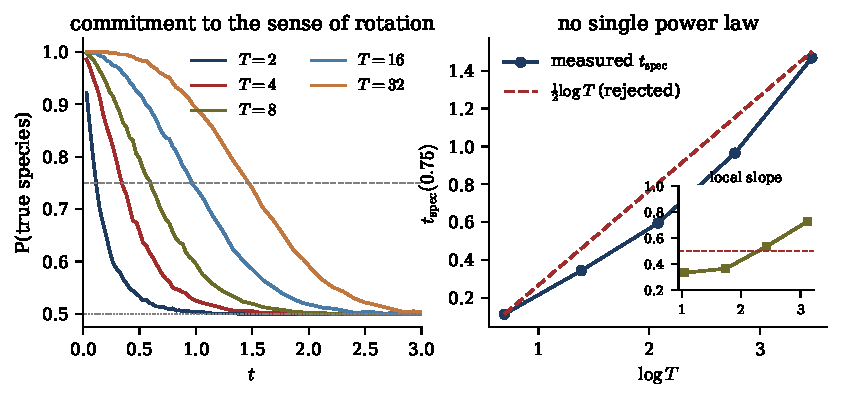
\includegraphics[width=\linewidth]{fig08_speciation.pdf}
\caption{Speciation in the sense of rotation, $\omega = 0.8$, $\sigma = 0.30$,
$4000$ trajectories per $T$, evaluated with the exact $\psi$-posterior. Left:
mean posterior probability of the true species against diffusion time; the
dashed line is the $0.75$ threshold defining $t_{\rm spec}$, the dotted line is
chance. Right: $t_{\rm spec}$ against $\log T$, with the $\tfrac12\log T$ law
that a first pass of this note asserted. It is rejected: the inset shows the
local slope drifting from $0.33$ to $0.72$ rather than sitting at $0.5$.}
\label{fig:spec}
\end{figure}

\subsection{Marginal blindness}

Finally the result that makes the per-frame/joint distinction sharp in this
model.

\begin{theorem}[Marginal blindness]\label{thm:blind}
For every frame $u$ and every diffusion time $t$, the single-frame marginal of
$P_t$ is rotationally symmetric in the plane and \emph{independent of $\psi$}.
Consequently the per-frame marginal score carries exactly zero information about
the rotation rate.
\end{theorem}

\begin{proof}
From \eqref{eq:chain},
$z_u = R_\psi^u z_0 + \sigma\sum_{k=1}^{u} R_\psi^{u-k}\eta_k$. Each
$R_\psi^{u-k}\eta_k$ is an isotropic Gaussian, hence equal in law to $\eta_k$,
and the terms stay independent; and $R_\psi^u z_0 \stackrel{d}{=} z_0$ because
$\theta_0$ is uniform. Therefore
\begin{equation}
  z_u \stackrel{d}{=} z_0 + \sigma\sqrt{u}\,\xi, \qquad \xi\sim\N(0,I_2),
\end{equation}
in which $\psi$ does not appear. Adding the isotropic channel preserves this.
\end{proof}

This is worth stating in words. The rotation rate is the entire content of the
model, and it is invisible to every single-frame marginal at every noise level.
Not harder to see --- invisible. A model trained on per-frame marginals cannot
represent the dynamics even in principle.

Figure~\ref{fig:jvm} is the consequence, and it is the practical point of the
whole note. Driving the reverse diffusion with the exact joint score reproduces
the data. Driving it with the sum of per-frame marginal scores --- which is a
perfectly valid score, namely that of the product of the marginals --- produces
frames whose radii are right to $1.3\%$ and whose turning angle is uniform. The
turning concentration is $0.009$ against a true rotation of $30^\circ$.

\begin{table}[b]\centering
\small
\begin{tabular}{lccc}
\toprule
& turning angle & concentration $R$ & radius, $u{=}0\to11$ \\
\midrule
data                              & $29.88^\circ$ & $0.959$ & $1.053 \to 1.350$\\
reverse SDE, exact joint score    & $30.07^\circ$ & $0.942$ & $1.058 \to 1.348$\\
reverse SDE, per-frame marginals  & ---           & $\mathbf{0.009}$ & $1.050 \to 1.334$\\
\bottomrule
\end{tabular}
\caption{Joint against marginal, $T = 12$, $D = 24$, $\sigma = 0.22$,
$\psi = 30^\circ$, $3000$ samples, $1500$ reverse-SDE steps. $R$ is the circular
concentration of the per-step turning angle. The marginal model matches every
single-frame statistic and has no dynamics at all: radii are not evidence.}
\label{tab:jvm}
\end{table}

\begin{figure}[t]\centering
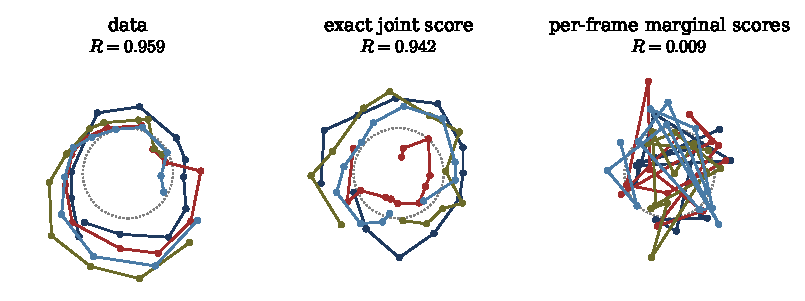
\includegraphics[width=\linewidth]{fig04_joint_vs_marginal.pdf}
\caption{Four trajectories from each of the three ensembles of
Table~\ref{tab:jvm}. Left: data. Middle: generated by the reverse SDE with the
exact joint score of Theorem~\ref{thm:score}, which also validates the closed
form end to end. Right: generated with per-frame marginal scores. The right
panel has the correct radial statistics and no rotation.}
\label{fig:jvm}
\end{figure}

%======================================================================
\section{Problem 2: the two-frame joint}\label{sec:p2}

\subsection{The model}

The board's middle panel: a scalar chain with additive drift,
\begin{equation}
  a_0 \sim P_0, \qquad a_1 = a_0 + c + \eta, \qquad \eta\sim\N(0,\sigma^2),
  \qquad
  q(x_0,x_1) = P_0(x_0)\,\N(x_1; x_0+c, \sigma^2),
  \label{eq:p2model}
\end{equation}
so $D = 2$. This is the minimal object whose joint score has a cross-frame
component at all.

\subsection{Gaussian prior: the gap is one number}

Take $P_0 = \N(\mu_0, v_0)$. Then $\E[a] = (\mu_0, \mu_0+c)$ and
\begin{equation}
  C_0 = \begin{pmatrix} v_0 & v_0 \\ v_0 & v_0 + \sigma^2\end{pmatrix},
\end{equation}
since $\mathrm{Cov}(a_0, a_1) = \mathrm{Cov}(a_0, a_0 + c + \eta) = v_0$ and
$\mathrm{Var}(a_1) = v_0 + \sigma^2$. The channel adds $\Delta$ to each
coordinate independently, so $P_t = \N(m\E[a], C_t)$ with
$C_t = m^2 C_0 + \Delta I$ and
\begin{equation}
  \score(x,t) = -C_t^{-1}\bigl(x - m\,\E[a]\bigr),
  \label{eq:p2score}
\end{equation}
which is the board's $-C_t^{-1}x + C_t^{-1}C_0\cdots e^{-t}$.

Now the key observation. The sum of the two per-frame marginal scores is
$-\mathrm{diag}(C_t)^{-1}(x - m\E[a])$, which is \emph{exactly diagonal at every
$t$}. So the entire difference between the joint object and the marginal object
is the single off-diagonal entry of $C_t^{-1}$. For a $2\times2$ matrix
$\begin{psmallmatrix}A&B\\B&C\end{psmallmatrix}$ the inverse has off-diagonal
$-B/\det$ with $\det = AC - B^2$, so putting $A = m^2v_0 + \Delta$,
$B = m^2 v_0$, $C = m^2(v_0+\sigma^2)+\Delta$,
\begin{align}
  \det &= (m^2v_0+\Delta)(m^2v_0 + m^2\sigma^2 + \Delta) - m^4v_0^2 \notag\\
       &= m^4 v_0\sigma^2 + 2\Delta m^2 v_0 + \Delta m^2 \sigma^2 + \Delta^2,
  \label{eq:p2det}
\end{align}
\begin{equation}
  \boxed{\ (C_t^{-1})_{01}
  = \frac{-m^2 v_0}
    {m^4 v_0\sigma^2 + 2\Delta m^2 v_0 + \Delta m^2\sigma^2 + \Delta^2}\ }
  \label{eq:p2coup}
\end{equation}

\subsection{The two limits, and a coefficient that had to be corrected}

\textbf{Large $t$.} As $t\to\infty$, $m\to0$ and $\Delta\to1$, so $\det \to 1$
and
\begin{equation}
  (C_t^{-1})_{01} \to -m^2 v_0 = -e^{-2t}v_0 .
\end{equation}
The coupling dies exponentially: \emph{temporal structure is a low-noise feature
of the score}, and it is the first thing corruption destroys.

\textbf{Small $t$.} Here one must be careful, because $m^2$ and $\Delta$ are not
independent: $m^2 = e^{-2t} = 1 - \Delta$ exactly. Substituting into
\eqref{eq:p2det},
\begin{align}
  \det &= (1-\Delta)^2 v_0\sigma^2 + 2\Delta(1-\Delta)v_0
        + \Delta(1-\Delta)\sigma^2 + \Delta^2 \notag\\
       &= v_0\sigma^2 + \Delta\bigl(-2v_0\sigma^2 + 2v_0 + \sigma^2\bigr)
        + O(\Delta^2)
        = v_0\sigma^2\Bigl[1 + \Delta\Bigl(-2 + \tfrac{2}{\sigma^2}
          + \tfrac{1}{v_0}\Bigr)\Bigr] + O(\Delta^2),
\end{align}
and with numerator $-(1-\Delta)v_0$,
\begin{equation}
  (C_t^{-1})_{01}
  = -\frac{1}{\sigma^2}(1-\Delta)
    \Bigl[1 - \Delta\Bigl(-2 + \tfrac{2}{\sigma^2} + \tfrac1{v_0}\Bigr)\Bigr]
    + O(\Delta^2)
  = -\frac{1}{\sigma^2}
    \Bigl[1 + \Delta\Bigl(1 - \tfrac{2}{\sigma^2} - \tfrac1{v_0}\Bigr)\Bigr]
    + O(\Delta^2).
  \label{eq:p2small}
\end{equation}
The limit $-1/\sigma^2$ is the innovation precision, as it must be. But note the
remainder prefactor: it is $2/\sigma^2 + 1/v_0 - 1$, \emph{not}
$2/\sigma^2 + 1/v_0$. The naive version --- which is what an earlier draft of
this note carried --- omits the $-1$ coming from $m^2 = 1-\Delta$, and is wrong
by $4.2\%$ at $\sigma^2 = 0.09$, $v_0 = 0.7$. The audit measures the ratio
across four decades of $\Delta$ and \emph{rejects} the naive coefficient. This
is the same failure mode as the factorial error caught in claim G8 of the main
ledger, and it is why coefficient audits are worth running.

Figure~\ref{fig:coup} shows the whole lifecycle.

\begin{figure}[t]\centering
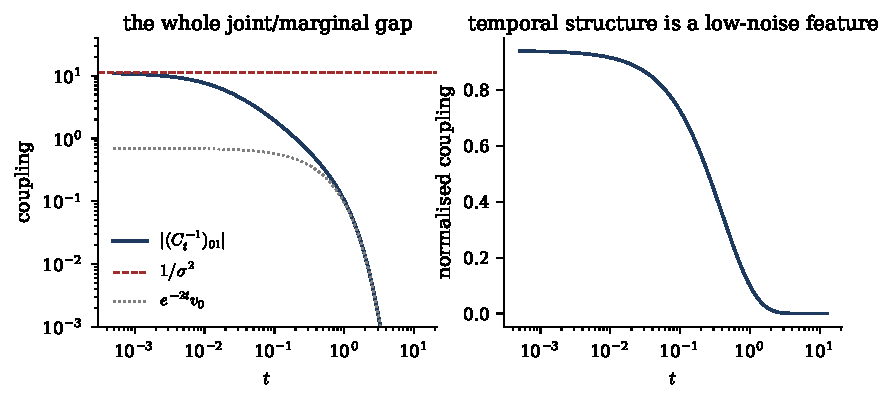
\includegraphics[width=\linewidth]{fig10_p2_coupling.pdf}
\caption{The coupling lifecycle, $v_0 = 0.7$, $\sigma^2 = 0.09$, $c = 1$. Left:
$|(C_t^{-1})_{01}|$ against $t$ with the two asymptotes $1/\sigma^2$ (dashed)
and $e^{-2t}v_0$ (dotted). Right: the same normalised by
$\sqrt{(C_t^{-1})_{00}(C_t^{-1})_{11}}$. Since the marginal object has zero
coupling at every $t$, these curves \emph{are} the joint/marginal gap.}
\label{fig:coup}
\end{figure}

\subsection{Mixture prior, and where speciation looks}

The board drew two bumps, so take $P_0 = \sum_k w_k \N(\mu_k, v)$. Conditionally
on component $k$ the pair $a$ is Gaussian with mean
$\nu_k = (\mu_k, \mu_k + c)$ and covariance
$\begin{psmallmatrix}v&v\\v&v+\sigma^2\end{psmallmatrix}$ --- the \emph{same}
for every $k$. So $P_t = \sum_k w_k \N(x; m\nu_k, C_t)$ with one shared $C_t$,
and
\begin{equation}
  \score(x,t) = \sum_k r_k(x)\,\bigl(-C_t^{-1}(x - m\nu_k)\bigr),
  \qquad r_k(x) \propto w_k\, \N(x; m\nu_k, C_t),
  \label{eq:p2mix}
\end{equation}
exact in $2\times2$ algebra. Which mode the reverse process picks is decided by
\begin{equation}
  \log\frac{r_1}{r_2} = \log\frac{w_1}{w_2}
  + m\,(\nu_1-\nu_2)\T C_t^{-1} x + \text{const},
\end{equation}
and since $\nu_1 - \nu_2 = (\mu_1-\mu_2)\one$, the $x$-dependence enters only
through $\one\T C_t^{-1}x$: \textbf{the discriminant is the frame average.} That
is the same mechanism as \eqref{eq:logoddsasym} --- averaging over frames raises
the effective signal-to-noise --- and it is why both problems have a speciation
time that grows with $T$. Figure~\ref{fig:p2field} shows the two score fields
side by side; this is the board's middle panel, drawn.

\begin{figure}[t]\centering
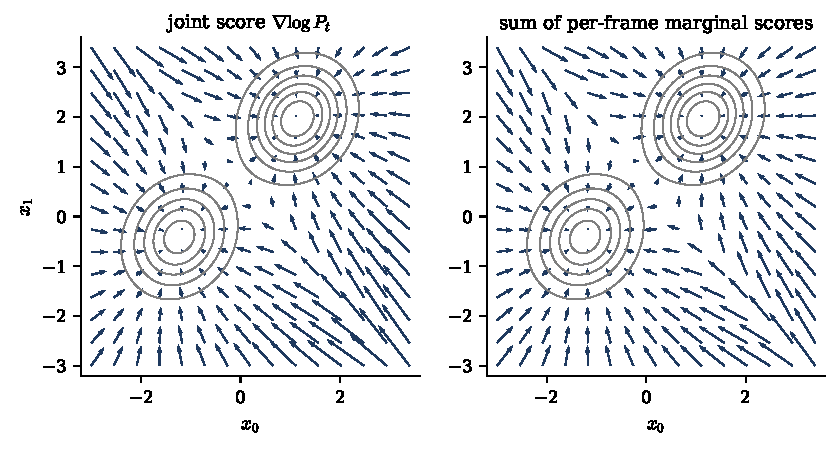
\includegraphics[width=\linewidth]{fig11_p2_field.pdf}
\caption{The board's middle panel. Two-bump prior
($\mu = \{-1.5, 1.4\}$, $w = \{0.45, 0.55\}$, $v = 0.10$), drift $c = 1$,
$\sigma = 0.30$, $t = 0.2$. Contours: $P_t(x_0,x_1)$. Arrows: left, the exact
joint score \eqref{eq:p2mix}; right, the sum of per-frame marginal scores. The
joint field tilts along the diagonal --- that tilt is the frame coupling, and it
is exactly what the marginal field lacks.}
\label{fig:p2field}
\end{figure}

\begin{remark}[Why Problem 1 is the better illustration]
In Problem 2 the drift $c$ \emph{is} visible in the marginals, since frame $1$
has mean $\mu_0 + c$. A per-frame model would get the drift roughly right and
only the correlation wrong. In Problem 1 the rotation is invisible to every
marginal (Theorem~\ref{thm:blind}). The difference is symmetry. So Problem 1 is
the model for making the per-frame/joint point, and Problem 2 is the model to
compute with.
\end{remark}

%======================================================================
\section{Problem 3: a reward on the last frame}\label{sec:p3}

\subsection{Control is tilting}

The board's right panel reads
$\E_{p_\mu}\bigl[-\int_0^1 |u(x,t)|^2\,\dd t - r(x_T)\bigr]$ with
$P(T) = f(\|x(T)-m\|^2/D)$. The control formulation and the tilting
formulation are the same thing, by the Gibbs variational principle: for any path
measure $Q$ absolutely continuous with respect to the uncontrolled reverse
process $P$,
\begin{equation}
  \E_Q[r] - \mathrm{KL}(Q \Vert P) \;\le\; \log \E_P\bigl[e^{r}\bigr],
  \qquad\text{with equality iff}\quad
  \frac{\dd Q}{\dd P} = \frac{e^{r}}{\E_P[e^r]}.
  \label{eq:gibbs}
\end{equation}
Since the quadratic control cost $\tfrac12\E\int\|v\|^2$ \emph{is} the KL
divergence to the uncontrolled process (Girsanov), the optimal terminal law is
simply the tilted prior
\begin{equation}
  P_0^r(a) \propto P_0(a)\, e^{r(a)} .
\end{equation}

Which SDE realises it? Define
\begin{equation}
  h_t(x) = \E\bigl[e^{r(a)} \,\big|\, x_t = x\bigr].
\end{equation}
Then the tilted process has marginals proportional to $P_t h_t$:
\begin{equation}
  P^r_t(x) \propto \int \dd a\, P_0(a)e^{r(a)}\N(x;ma,\Delta I)
  = P_t(x)\int \dd a\, p(a\mid x)\, e^{r(a)} = P_t(x)\, h_t(x).
  \label{eq:htransform}
\end{equation}
So the optimally controlled reverse SDE is the ordinary one with score
$\nabla\log(P_t h_t)$: the extra drift is $g^2\nabla \log h_t$, which with
$g^2 = 2$ is the board's $u_{\rm optimal} \approx 2f$. This is Doob's
$h$-transform.

\subsection{Everything in closed form for a quadratic reward}

Take $P_0 = \N(0, C_0)$ on the trajectory, $E$ the selector of the last frame,
and $r(a) = -\|Ea - m_*\|^2/2s^2$ --- the quadratic choice of the board's $f$.

\textbf{The tilted prior.} Multiplying two Gaussians adds precisions:
\begin{equation}
  C_0^r = \bigl(C_0^{-1} + E\T E/s^2\bigr)^{-1}
        = C_0 - C_0 E\T\bigl(s^2 + E C_0 E\T\bigr)^{-1} E C_0,
  \qquad \mu_0^r = C_0^r E\T m_*/s^2,
  \label{eq:tilted}
\end{equation}
the second form by Woodbury.

\textbf{The value function.} The posterior of the clean trajectory is
$a\mid x \sim \N(\mu_p, \Sigma_p)$ with
\begin{equation}
  \Sigma_p = \bigl(C_0^{-1} + (m^2/\Delta) I\bigr)^{-1},
  \qquad \mu_p = \Sigma_p (m/\Delta)\, x .
\end{equation}
Only $y = Ea$ matters, and $y \sim \N(\nu_t, S_t)$ with $\nu_t = E\mu_p$,
$S_t = E\Sigma_p E\T$. A Gaussian expectation of a Gaussian gives
\begin{equation}
  \log h_t(x) = -\tfrac12\log\bigl|I + S_t/s^2\bigr|
  - \tfrac12 (\nu_t - m_*)\T (S_t + s^2 I)^{-1}(\nu_t - m_*),
  \label{eq:logh}
\end{equation}
and since $\nu_t$ is linear in $x$,
\begin{equation}
  \nabla_x \log h_t(x)
  = -\frac{m}{\Delta}\, \Sigma_p E\T (S_t + s^2 I)^{-1}(\nu_t - m_*).
  \label{eq:gradlogh}
\end{equation}
Running the reverse SDE with this extra drift reproduces $\N(\mu_0^r, C_0^r)$ to
$0.2\%$ in the mean and $1.3\%$ in the covariance.

\subsection{How far back does the reward reach?}

This is the board's $P(\tau) \Leftarrow P(T)$, and \eqref{eq:tilted} answers it
exactly. Taking the diagonal of the Woodbury form, with $E$ selecting the last
frame,
\begin{equation}
  \boxed{\ C_0^{(uu)} - C_0^{r,(uu)}
  = \frac{\bigl(C_0^{(u,T-1)}\bigr)^2}{s^2 + C_0^{(T-1,T-1)}}\ }
  \label{eq:reach}
\end{equation}
The reward propagates backwards \emph{along the covariance function of the
prior}, and nothing else. The two models of this project bracket the behaviour:

\begin{itemize}[leftmargin=1.4em, itemsep=2pt]
\item \textbf{ring-anchored walk}, $C_0^{(uv)} = \rho_0 + \sigma^2\min(u,v)$:
      the reduction is nonzero for \emph{every} $u$ and grows with $u$. A
      constraint on the last frame reshapes the whole trajectory.
\item \textbf{stationary AR(1)} of the main thesis, $C_0^{(uv)} =
      \alpha^{|u-v|}$: the reduction decays by exactly $\alpha^2$ per frame
      going backwards, with range $\xi = 1/\log(1/\alpha)$. This is the $q^r$
      locality law (claim G12) reappearing.
\end{itemize}

At $T = 16$, $\alpha = 0.8$, $s^2 = 0.25$ the two differ by more than two orders
of magnitude at the first frame. \emph{Non-stationary priors propagate a
terminal reward globally; stationary ones propagate it over a finite memory.}
Figure~\ref{fig:reach} shows both, together with the board's ellipse sketch at
$T = 2$.

\begin{figure}[t]\centering
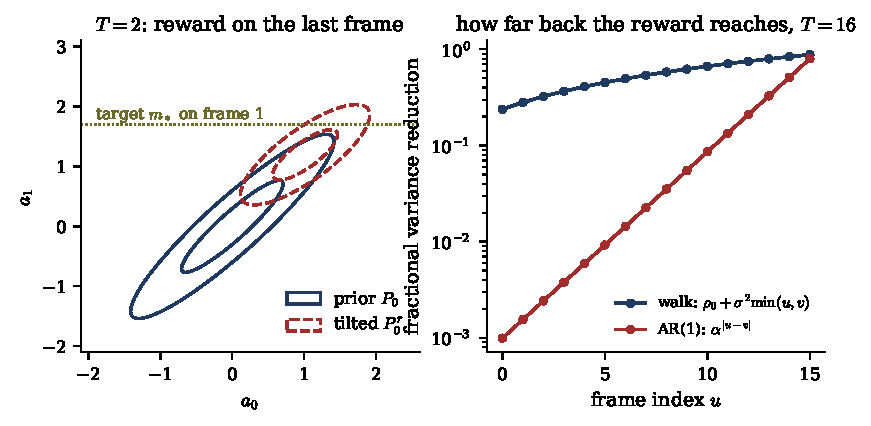
\includegraphics[width=\linewidth]{fig12_p3_reach.pdf}
\caption{Left: the board's ellipse picture at $T = 2$. One- and two-sigma
ellipses of the prior $P_0 = \N(0, C_0)$ and of the tilted law $P_0^r$ after a
quadratic reward pulls frame $1$ towards $m_* = 1.7$ ($s^2 = 0.25$). The ellipse
contracts along $a_1$ and shifts in \emph{both} coordinates --- the constraint
propagates to frame $0$ through the prior correlation. Right: the reach
\eqref{eq:reach} at $T = 16$ for the two priors, as a fraction of the prior
variance of each frame, on a log scale.}
\label{fig:reach}
\end{figure}

%======================================================================
\section{Two claims that measurement rejected}\label{sec:rejected}

A first pass of this note asserted two scaling laws by argument rather than
measurement. Both are false. They are recorded here, with the rejection under
test, so they cannot creep back.

\subsection{H1: \texorpdfstring{$t_{\rm spec} = \tfrac12\log T$}{t spec = half log T} --- rejected}

The argument was that the sense of rotation is encoded redundantly across
neighbouring frame pairs, so the evidence grows like $T$, the log-odds like
$e^{-2t}T$, and hence $t_{\rm spec} \simeq \tfrac12\log T$. Measured with the
exact $\psi$-posterior:

\begin{center}\small
\begin{tabular}{lcccccc}
\toprule
$T$ & 2 & 4 & 8 & 16 & 32 & 64\\
$t_{\rm spec}(0.75)$ & $0.11$ & $0.34$ & $0.59$ & $0.96$ & $1.45$ & $2.05$\\
local slope & \multicolumn{1}{c}{} & $0.33$ & $0.37$ & $0.53$ & $0.71$ & $0.86$\\
\bottomrule
\end{tabular}
\end{center}

\noindent
$t_{\rm spec}$ does rise with $T$, but the local slope
$\dd t_{\rm spec}/\dd\log T$ drifts monotonically from $0.33$ to $0.86$. There
is no single power law over this range, and $\tfrac12$ is not the slope anywhere
except by coincidence near $T = 8$. The likely cause of the drift is that
$K_{uv} = \min(u,v)$ is non-stationary: neighbouring-pair terms carry weight
$u$, so they sum to $\sim T^2/2$ rather than $\sim T$, and the effective
exponent crosses over as $T$ grows.

\textbf{Left open.} The asymptotic law. At large $t$ the $T$-exponent of the
log-odds measures between $2.7$ and $3.2$ and the $e^{-2t}$ prefactor law does
not hold cleanly there, so no clean asymptotic form is claimed. Ground truth
exists at any $T$ by Proposition~\ref{prop:mix}, so this is a measurement
waiting to be done, not a derivation.

\subsection{H2: \texorpdfstring{$\Theta(T^2)$}{Theta(T2)} versus \texorpdfstring{$O(1)$}{O(1)} samples --- rejected}

The argument was the board's own parameter count: an unstructured joint
Gaussian score has $D(D+1)/2$ free parameters against $O(1)$ for the structured
version, so the sample requirement should be $\Theta(T^2)$ against $O(1)$.

This is false at any fixed $t$, and the reason is instructive: \textbf{the
diffusion's own noise floor $\Delta_t$ regularises the empirical score.} Since
$\hat C_t = m^2 \hat C_0 + \Delta I$, even a badly estimated or rank-deficient
$\hat C_0$ gives a usable score as long as $\Delta$ is not small. Measured in
the Gaussian surrogate at $T = 8$, $D = 16$ (so $D(D+1)/2 = 136$), for a $10\%$
relative score error:

\begin{center}\small
\begin{tabular}{lccccccc}
\toprule
$t$ & $0.02$ & $0.035$ & $0.05$ & $0.1$ & $0.2$ & $0.4$ & $0.8$\\
$\Delta_t$ & $0.039$ & $0.068$ & $0.095$ & $0.181$ & $0.330$ & $0.551$ & $0.798$\\
$N$ unstructured & $576$ & $374$ & $242$ & $126$ & $66$ & $28$ & $18$\\
$N$ structured & $18$ & $18$ & $18$ & $18$ & $18$ & $18$ & $18$\\
ratio & $32.0$ & $20.8$ & $13.4$ & $7.0$ & $3.7$ & $1.6$ & $1.0$\\
$N\Delta/D$ & $1.41$ & $1.58$ & $1.44$ & $1.43$ & $1.36$ & $0.96$ & $0.90$\\
\bottomrule
\end{tabular}
\end{center}

\noindent
so the measured law is
\begin{equation}
  N_{\rm unstructured} \;\approx\; 1.46\,(\pm 0.07)\ \frac{D}{\Delta_t}
  \qquad \text{for } \Delta_t \lesssim 0.2,
  \label{eq:h2law}
\end{equation}
saturating to $N \sim O(D)$ at large $\Delta_t$; and the $D$-exponent at
$t = 0.05$ measures $0.69$--$0.89$ across seeds, sub-linear to linear and
definitively not $D^2$. The structured estimator --- the gauge plus the two
scalars $\rho_0, \sigma^2$ --- needs $N = 18$ at every noise level.

So the board's $N > D(D+1)/2$ is a parameter count for identifying $C_0$
\emph{itself}, which is strictly stronger than what an accurate score at
$t > 0$ requires. The real content of the panel is that the structured/
unstructured gap is set by the noise level and opens only as $t \to 0$ --- which
is exactly the memorisation regime, and therefore exactly where to look next.
Figure~\ref{fig:h2} shows both laws.

\begin{figure}[t]\centering
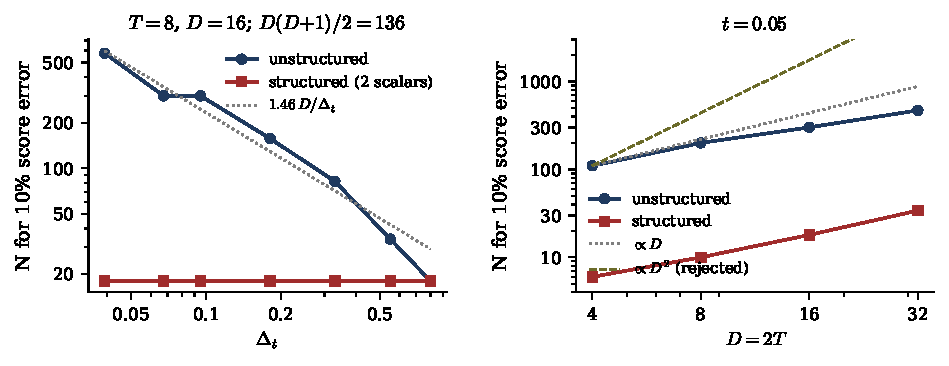
\includegraphics[width=\linewidth]{fig14_h2.pdf}
\caption{Sample complexity in the Gaussian surrogate, for a $10\%$ relative
joint-score error. Left: against the noise floor $\Delta_t$ at $T = 8$, with
\eqref{eq:h2law} dotted. Right: against dimension at $t = 0.05$, with
$\propto D$ dotted and the rejected $\propto D^2$ dashed. The structured
estimator is flat in $\Delta_t$; the gap between the two is a function of the
noise level, not of $T$.}
\label{fig:h2}
\end{figure}

%======================================================================
\section{What is verified, and how}\label{sec:audit}

Every closed-form claim is checked against an independently computed reference
--- polar Gauss--Legendre quadrature of the exact mixture, central finite
differences of $\log P_t$, brute-force linear algebra, or Monte Carlo --- in the
protocol of the main thesis appendix. One command runs everything:

\begin{center}\ttfamily
python code/run\_all.py \qquad $\longrightarrow$ \qquad 66 checks
\end{center}

\noindent
and it exits non-zero on any failure.

\begin{table}[h]\centering
\footnotesize
\setlength{\tabcolsep}{4pt}
\begin{tabular}{llll}
\toprule
\# & Claim & Class & Evidence \\
\midrule
R1  & rotation is an orthogonal gauge (Lem.~\ref{lem:gauge})    & EXACT & $1.4\times10^{-17}$\\
R2  & joint score $=$ linear $+$ rank one (Thm.~\ref{thm:score})& EXACT & vs finite diff.\ $4\times10^{-10}$\\
R2b & correction is $m\E[z_0|x]$, rank exactly $1$ (Prop.~\ref{prop:anchor}) & EXACT & $2\times10^{-15}$\\
R3  & random $\psi$: posterior average, any $T$ (Prop.~\ref{prop:mix}) & EXACT & $8.9{\times}10^{-10}$; $7.7{\times}10^{-10}$ at $T{=}3$\\
R3a & $p(\psi|x,t)\propto p(\psi)\Z_t(\beta)$, \emph{$T{=}2$ only} (Rem.~\ref{rem:scope}) & EXACT, scoped & $1.8{\times}10^{-16}$; fails $T{\ge}3$\\
R4  & $\beta(\psi)$ identity, peak at $\gamma$ (Prop.~\ref{prop:T2}) & EXACT & $8.9\times10^{-16}$\\
R5  & two-species log-odds \eqref{eq:logoddsasym} & EXACT (asympt.) & $0.2\%$ at three $t$\\
R6  & marginal blindness (Thm.~\ref{thm:blind}) & EXACT & proof $+$ MC $3.7\times10^{-3}$\\
R7  & two-frame score; marginal object diagonal \eqref{eq:p2score} & EXACT & $2.8\times10^{-11}$\\
R8  & coupling \eqref{eq:p2coup}; prefactor $2/\sigma^2{+}1/v_0{-}1$ & EXACT & $4.4\times10^{-4}$; naive rejected\\
R9  & mixture score \eqref{eq:p2mix}; frame-average discriminant & EXACT & $8.6\times10^{-11}$\\
R11 & Gaussian $h_t$, $\nabla\log h_t$; controlled SDE & EXACT $+$ NUM. & $8{\times}10^{-11}$; SDE $0.2\%$ / $1.3\%$\\
R12 & reward reach \eqref{eq:reach} & EXACT & $3.3\times10^{-16}$\\
R13 & $N_{\rm uns}\approx1.46\,D/\Delta_t$ \eqref{eq:h2law} & NUMERICAL & $c$ stable to $12\%$\\
R14 & band structure of $A_t^{-1}$ (Prop.~\ref{prop:band}) & EXACT & decoupling $0$; band law $19\%$\\
\midrule
\sout{H1} & \sout{$t_{\rm spec} = \tfrac12\log T$} & \textbf{REJECTED} & slope drifts $0.33\to0.86$\\
\sout{H2} & \sout{$\Theta(T^2)$ vs $O(1)$ samples} & \textbf{REJECTED} & $D$-exponent $0.69$--$0.89$\\
O1  & asymptotic $t_{\rm spec}(T)$ law & OPEN & exponent $2.7$--$3.2$, unclean\\
\bottomrule
\end{tabular}
\caption{The ledger. Classes as in the main thesis \texttt{RESULT\_LEDGER.md}:
EXACT means closed form with a numerical audit, NUMERICAL means measured against
a validated reference with no closed form.}
\label{tab:ledger}
\end{table}

The figures are generated by \texttt{note/make\_note\_figures.py}, which imports
its model functions from the audited driver and re-checks the closed-form score
against finite differences before plotting anything.

%======================================================================
\section{Where this leaves things}\label{sec:next}

Three results are worth carrying forward.

\textbf{The board's circle model is exactly solvable.} Between
Lemma~\ref{lem:gauge}, Theorem~\ref{thm:score} and Proposition~\ref{prop:mix}
there is ground-truth joint score at any $T$ from two nested one-dimensional
integrals. Chapter~6 of the thesis currently records these models as having ``no
closed form for their joint score in reach'' and as ``set aside, deliberately
and explicitly''; that is too pessimistic and the passage needs rewriting.

\textbf{Marginal blindness is the clean statement of the per-frame error.}
Theorem~\ref{thm:blind} says the rotation rate is invisible to every single-frame
marginal at every noise level. Table~\ref{tab:jvm} shows what that costs in
practice. Because the ring marginal is visibly non-Gaussian and \emph{still}
blind, this is a better illustration than the stationary Gaussian chain, where
the marginal score is the trivial $-x_k$.

\textbf{Structure matters at low noise, not at high dimension.} Equation
\eqref{eq:h2law} relocates the finite-sample question. The interesting regime is
small $\Delta_t$, which is the memorisation regime, and the natural next step is
the rest of the board's finite-$N$ panel: the Gram-matrix conditions and the
collapse transition proper.

Two smaller items remain open: the asymptotic $t_{\rm spec}(T)$ law (O1), and
whether $p(\psi)$ should be continuous --- the von Mises picture of
Proposition~\ref{prop:T2} --- or two-species --- the speciation picture of
\eqref{eq:logoddsasym} --- as the primary object.

\end{document}
